\documentclass[pdf]{beamer}

%\mode<presentation>{\usetheme{Warsaw}}

\usepackage{pgfpages}
%\setbeameroption{show notes on second screen}

\usepackage[utf8]{inputenc}
\usepackage{xeCJK}
\usepackage{tikz-cd}
\usepackage{graphicx}
\usepackage {mathtools}
\usepackage{utopia} %font utopia imported
\usetheme{Ilmenau}
\usepackage{caption}
\usepackage{subcaption}
\usepackage[french]{babel}
\usepackage{quiver}
\tikzcdset{scale cd/.style={every label/.append style={scale=#1},cells={nodes={scale=#1}}}}


% set colors
\definecolor{myNewColorA}{RGB}{46,139,87} % eric orange
\definecolor{myNewColorB}{RGB}{169,169,169} 
\definecolor{myNewColorC}{RGB}{46,139,87} 
\setbeamercolor*{palette primary}{bg=myNewColorC}
\setbeamercolor*{palette secondary}{bg=myNewColorB, fg = white}
\setbeamercolor*{palette tertiary}{bg=myNewColorA, fg = white}
\setbeamercolor*{titlelike}{fg=myNewColorA}
\setbeamercolor*{title}{bg=myNewColorA, fg = white}
\setbeamercolor*{item}{fg=myNewColorA}
\setbeamercolor*{caption name}{fg=myNewColorA}
\usefonttheme{professionalfonts}

\usepackage[style=ieee]{biblatex}
\usepackage{hyperref}

\setbeamertemplate{bibliography item}{\insertbiblabel}
\addbibresource{references.bib}

%------------------------------------------------------------

%\titlegraphic{\includegraphics[width=3cm]{}} 

\setbeamerfont{title}{size=\large}
\setbeamerfont{subtitle}{size=\small}
\setbeamerfont{author}{size=\small}
\setbeamerfont{date}{size=\small}
\setbeamerfont{institute}{size=\small}
\beamertemplatenavigationsymbolsempty
%\defbeamertemplate*{headline}{myminiframes theme}
%{

%}
\defbeamertemplate*{footline}{myminiframes theme}
  {%
    \begin{beamercolorbox}[colsep=1.5pt]{upper separation line foot}
    \end{beamercolorbox}
    %\begin{beamercolorbox}[ht=2.5ex,dp=1.125ex,%
    %  leftskip=.3cm,rightskip=.3cm plus1fil]{author in head/foot}%
    %  \leavevmode{\usebeamerfont{author in head/foot}\insertshortauthor}%
    %  \hfill%
    %  {\usebeamerfont{institute in head/foot}\usebeamercolor[fg]{institute in head/foot}\insertshortinstitute}%
    %\end{beamercolorbox}%
    \begin{beamercolorbox}[ht=2.5ex,dp=1.125ex,%
      leftskip=.3cm,rightskip=.3cm plus1fil]{title in head/foot}%
      {\usebeamerfont{title in head/foot}\insertshorttitle\hfill \insertframenumber/\inserttotalframenumber}%<-here
    \end{beamercolorbox}%
    \begin{beamercolorbox}[colsep=1.5pt]{lower separation line foot}
    \end{beamercolorbox}
  }
\makeatother

\title{Graphe de proximité sémantique de la langue française}
\subtitle{Proposé par AINÜW}

\date[\textcolor{white}{16 Nov 2023}]  %% Change presentation date here
{\today}

\author[Equipe AINUW]{Equipe AINÜW}
%\institute[13e IPSW]{\inst{1} affiliation for author1 \and %
%                     \inst{2} affiliation for author2}

%\logo{
%\includegraphics[width=2cm]{images/CRM.png}
%}

%------------------------------------------------------------
%This block of commands puts the table of contents at the 
%beginning of each section and highlights the current section:
%\AtBeginSection[]
%{
%  \begin{frame}
%    \frametitle{Contents}
%    \tableofcontents[currentsection]
%  \end{frame}
%}
%------------------------------------------------------------

\begin{document}

%The next statement creates the title page.
\frame{\titlepage}
\begin{frame}
\frametitle{Contents}
\tableofcontents
\end{frame}
%------------------------------------------------------------
\section{Introduction}
    \begin{frame}{Problématique}
    % \begin{center}    
    Conception d'un outil de profilage des systèmes (tout est système !): Analyse des réponses d'un utilisateur à un formulaire dans le but de déterminer les concepts de la langue française  auquel se rattache l'utilisateur dans le but d'évaluer la compatibilité entre 2 systèmes.
    % \end{center}
    \end{frame}

    \begin{frame}{Formalisation}
    \begin{enumerate}
        \item Génération d'un graphe de concepts sous-jacent pour la langue française.
        \item Analyse d'un utilisateur afin de déterminer les concepts dans lesquels ils se reconnaît.
    \end{enumerate}
    \end{frame}

    \begin{frame}{Exemple:}
    \begin{center}
        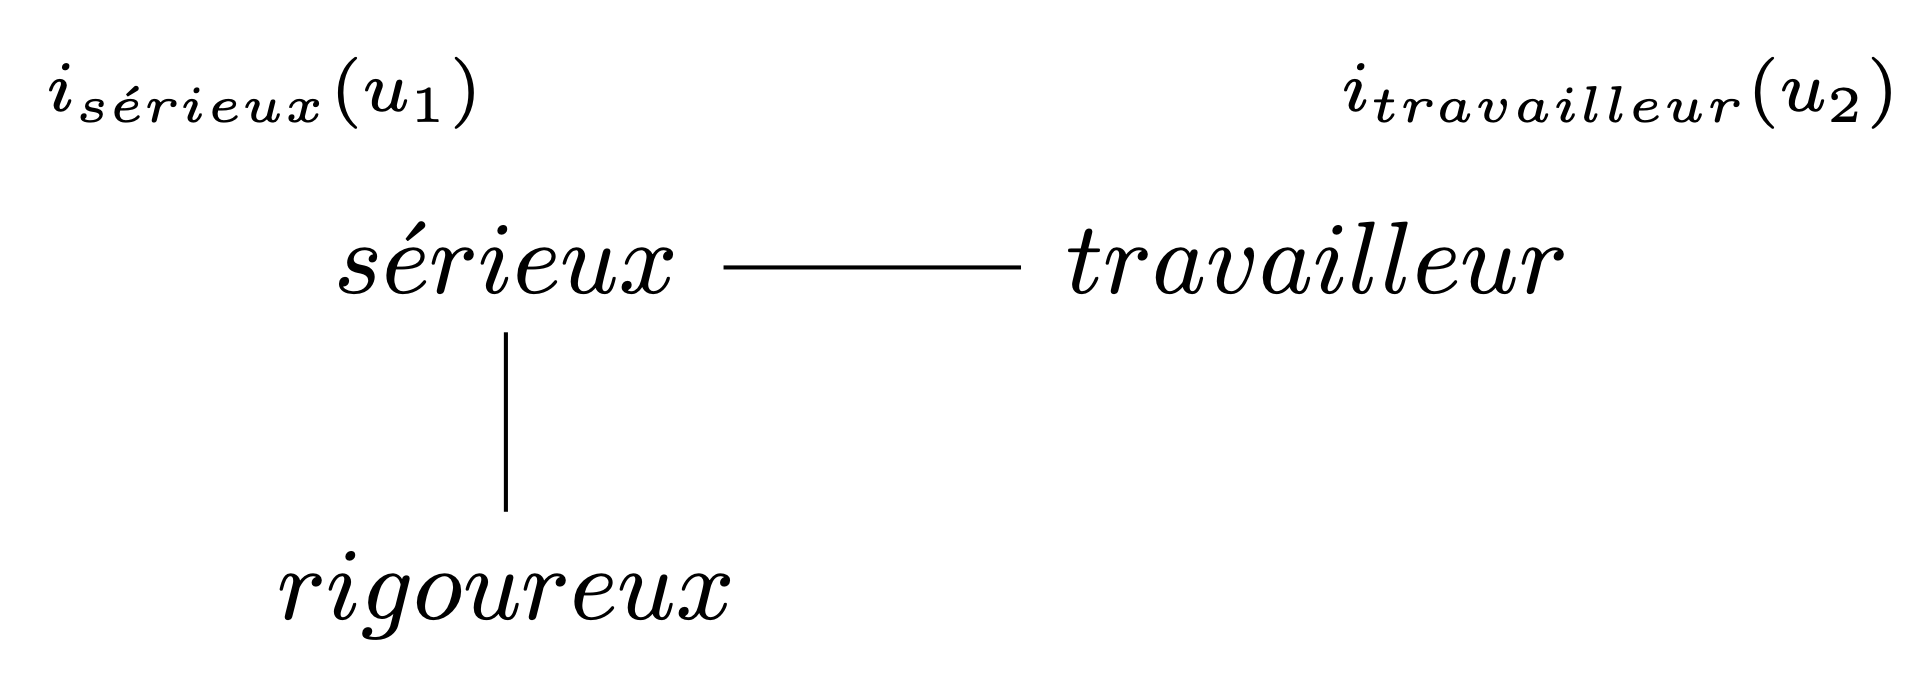
\includegraphics[scale = 0.30]{Images/image_graphe_ex.png}
    \end{center}
    % \begin{equation}
    %     Compatibilité(u_1, u_2) = \Sigma
    % \end{equation}
    
    \end{frame}

\section{Approche}

\begin{frame}{Approche}
    On se concentre sur 1.
    \textbf{Comment fabrique-t-on le graphe ?}
    Génération d'un graphe de concepts, où les noeuds sont des concepts de la langue française et les arcs entre deux noeuds représentent une relation de proximité sémantique.
\end{frame}

\begin{frame}{Remarques}
        \textit{Remarque 1:} On pourrait penser à d'autres types de relations entre les concepts: 
    \begin{itemize}
        \item synonymie,
        \item antonymies,
        \item taxonomie\dots
    \end{itemize}
    \textit{Remarque 2:} Un mot peut désigner plusieurs concepts.
    
    \textit{Remarque 3:} Un concept est représenté par une unique définition.

    \textbf{Comment obtenir des concepts à partir d'une collection de mots ?}

    \textbf{Comment évaluer la proximité sémantique entre deux concepts ?}
\end{frame}

\begin{frame}{Description de la méthode}
\begin{enumerate}
    \item Utilisation de la bibliothèque \textit{NLTK} et de son module \textit{Wordnet} pour récupérer les concepts et leur définition,
    
    \textit{Remarque:} Attention, les concepts et leur définition sont définis en anglais: traduction avec la bibliothèque google translate.
    \item On utilise une bibliothèque de NLP contextuelle pré-entrainée conçue en tant qu'algorithme génératif: générer à partir d'une phrase une représentation vectorielle de cette phrase.

    On se tourne vers le modèle CamemBERT qui est pré-entrainé sur un corpus français.
\end{enumerate}
\end{frame}

\begin{frame}{Description d'un méthode}
    On donne à CamemBERT les définitions de deux concepts. On mesure une distance entre leurs représentations vectorielles et cela nous donne un score de similarité et on décide d'un seuil à partir duquel deux mots sont liés sémantiquement. 
\end{frame}

\section{Résultats préliminaires}
    \begin{frame}{Résultat:}
    On teste notre méthode sur les mots \textbf{orange et voiture} qui engendrent 14 concepts !
    \begin{center}
        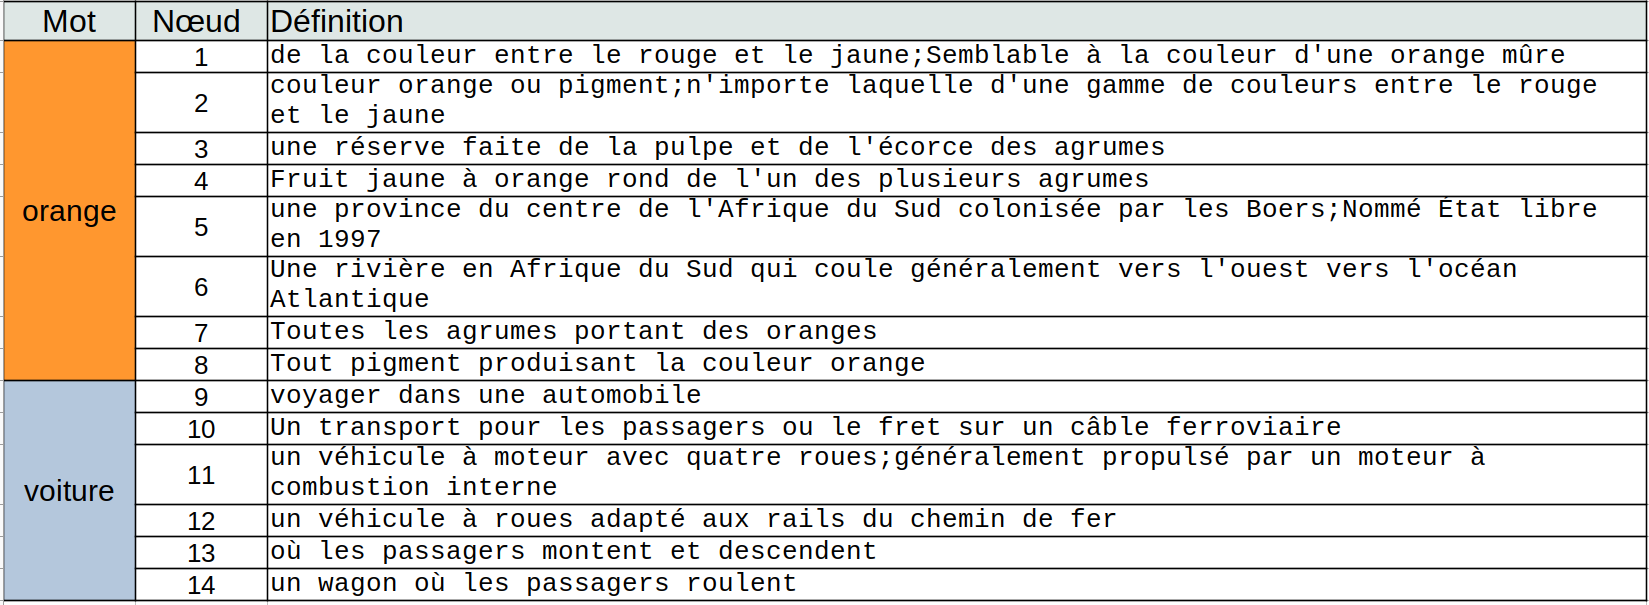
\includegraphics[scale = 0.175]{Images/def_mot.png}
    \end{center}
    % \begin{equation}
    %     Compatibilité(u_1, u_2) = \Sigma
    % \end{equation}
    
    \end{frame}

    \begin{frame}{Résultats:}
    \begin{center}
        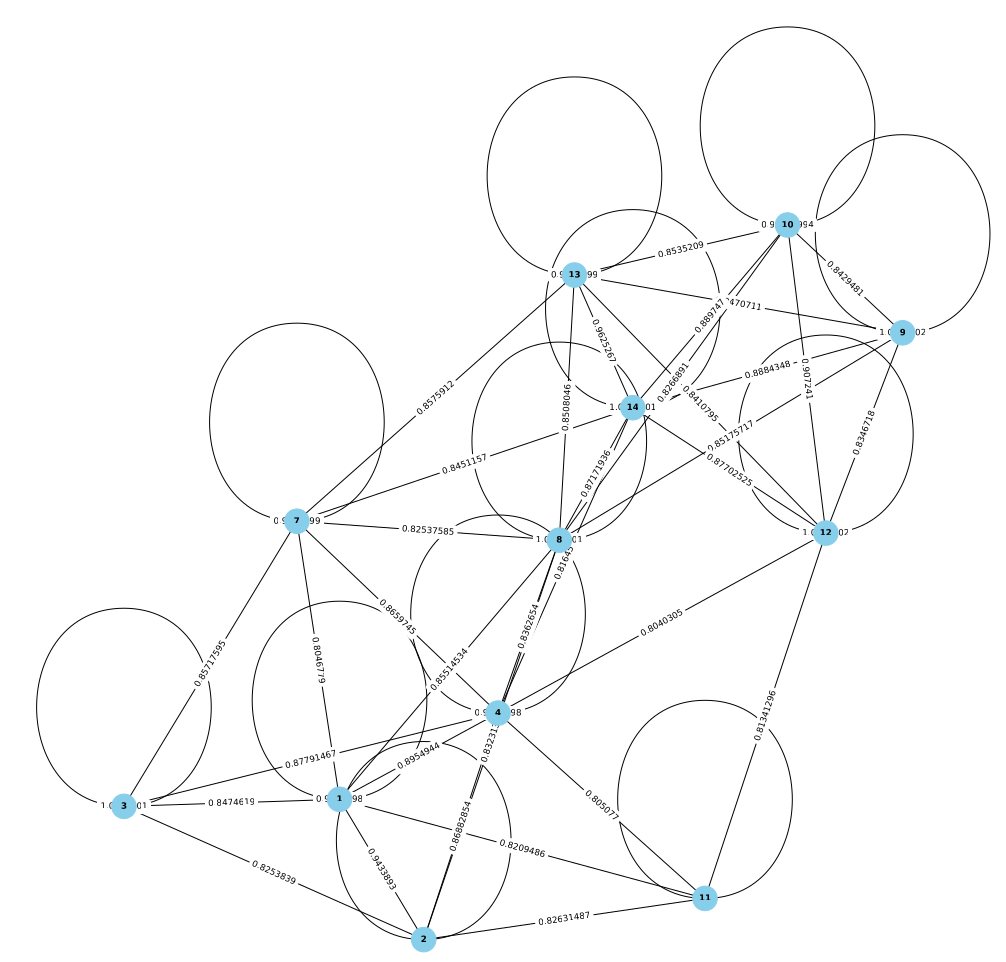
\includegraphics[scale = 0.18]{Images/graphe_pt1.png}
        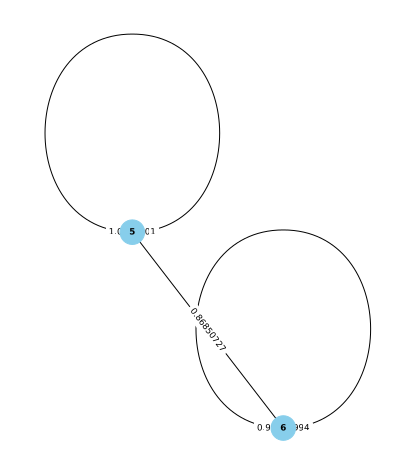
\includegraphics[scale = 0.18]{Images/graphe_pt2.png}
    \end{center}
    % \begin{equation}
    %     Compatibilité(u_1, u_2) = \Sigma
    % \end{equation}
    
    \end{frame}


\section{Conclusion}
    \begin{frame}{Limitations de notre méthode}
\begin{enumerate}
    \item Le fait de passer par un traducteur ajoute du biais,
    \item Une étude doit être faite sur le choix du seuil,
    \item Choix des mots,
    \item Besoin de ressources pour calculer les représentations vectorielles.
\end{enumerate}
\end{frame}

\begin{frame}{Perspectives}
\begin{enumerate}
    \item Utiliser un dictionnaire français pour éviter l'utilisation d'un traducteur,
    \item Augmentation du corpus avec les mots signifiants les plus fréquents de la langue française,
    \item Fine-tuner CamemBERT sur un corpus [mots, définitions],
    \item Benchmarker le choix du seuil,
    \item Traiter d'autres relations que la relation sémantique.
\end{enumerate}
    \end{frame}

\section*{}
\begin{frame}
\textcolor{myNewColorA}{\Huge{\centerline{Merci !}}}
\end{frame}

% \begin{frame}[noframenumbering]{References}
% \printbibliography
% \end{frame}

\end{document}